\section{Force estimation}
%%%%%%%%%%%% MID WAY AGENDA %%%%%%%%%%%%%%

\begin{frame}{Force estimation}{Overview}
\begin{itemize}
  	\item Roll, pitch and yaw forces
\end{itemize}
 \begin{figure}[h]
 \centering
 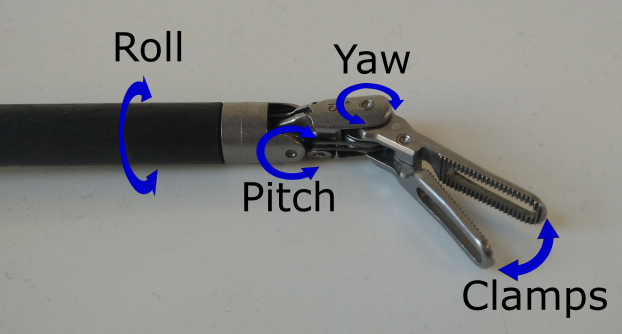
\includegraphics[scale = 0.5]{Endowrist31}
 \label{fig:ewr}
 \end{figure}
\end{frame}

\begin{frame}{Force estimation}{Overview}
\begin{itemize}
\item Nonlinearities in the EndoWrists dynamics caused by inter wire friction and elasticity
\begin{itemize}
\item Analytical model exists, but requires parameter identification
\item Not possible to replicate the data acquisition process using our setup
\end{itemize}
\item Model is fitted to data acquired with our setup
\end{itemize}
\end{frame}

\begin{frame}{Force estimation}{Data acquisition}
\begin{itemize}
\item Yaw and Pitch force measurement made with load cell setup
\begin{itemize}
\item Load cell output read by Arduino logged by SBrio
\item Position, velocity, current (effort) and setpoints logged by SBrio
\end{itemize}
\item Measurement process slow and prone to error
\begin{itemize}
\item Disturbances in data
\end{itemize}
\end{itemize}
\begin{figure}
\centering
    \begin{subfigure}[t]{0.32\textwidth}
        \centering
        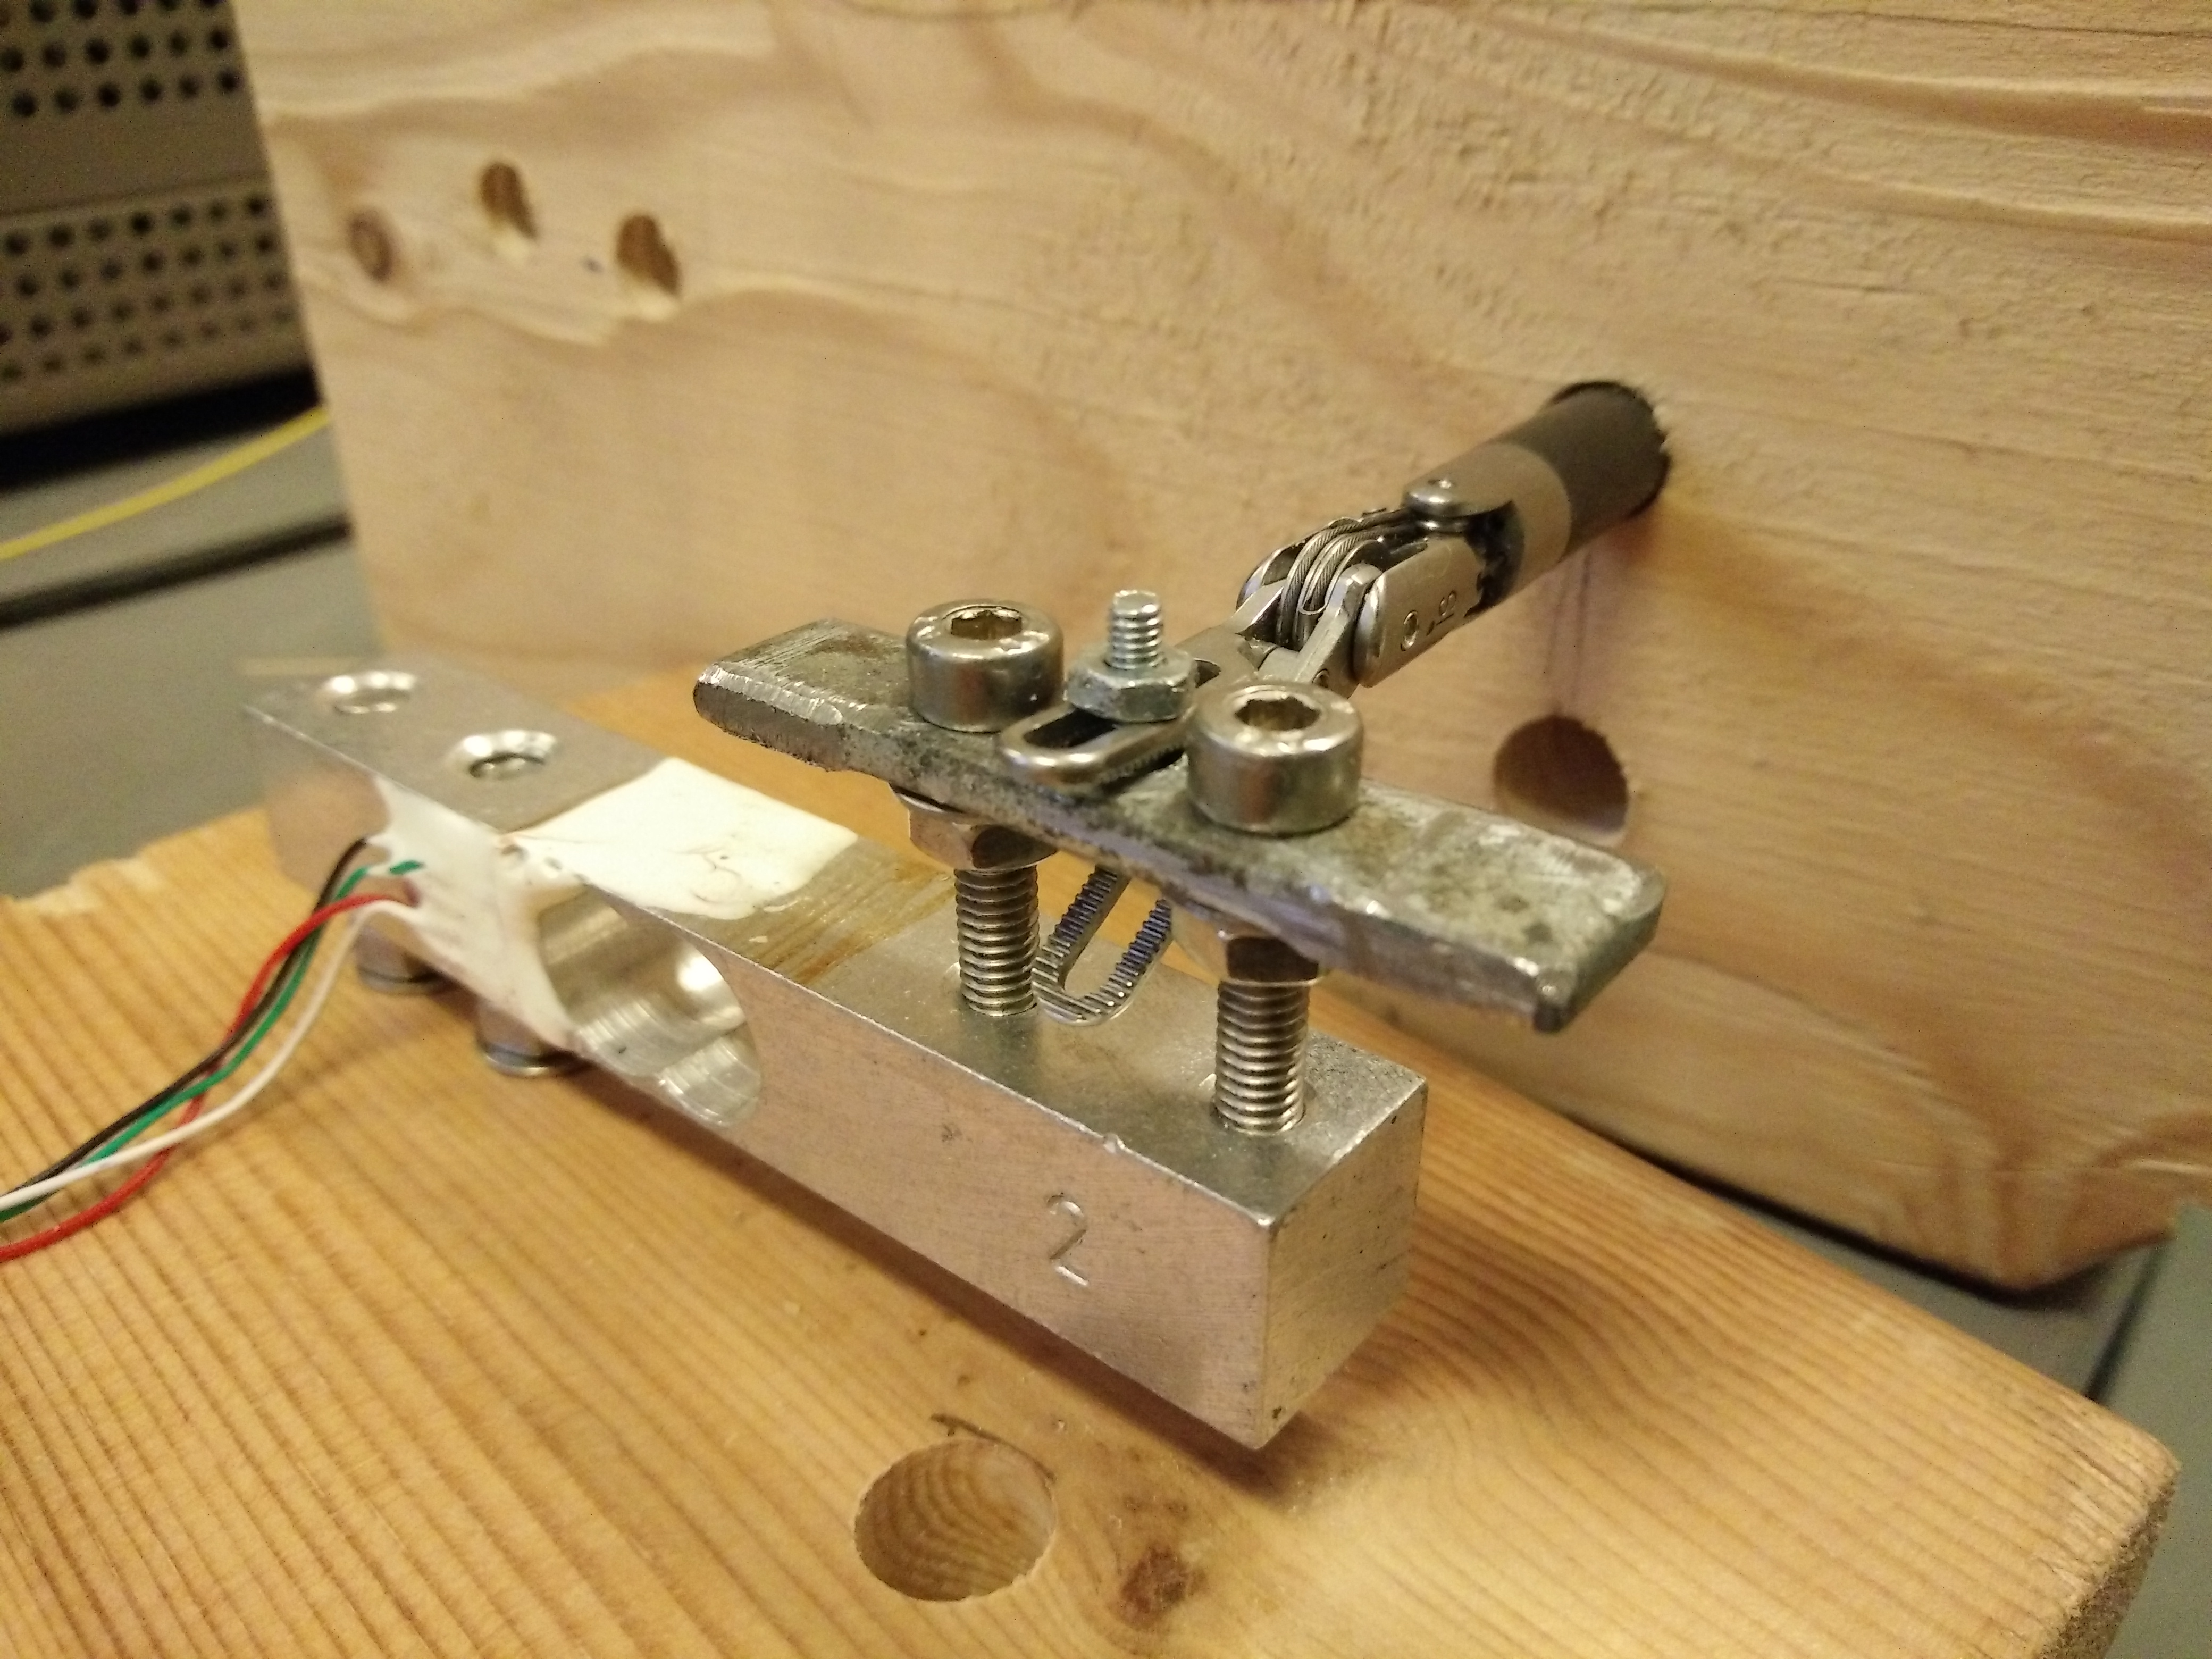
\includegraphics[width=\linewidth]{One_clamp.jpg} 
        \caption{Yaw} \label{fig:mes1}
    \end{subfigure}
    \begin{subfigure}[t]{0.32\textwidth}
        \centering
        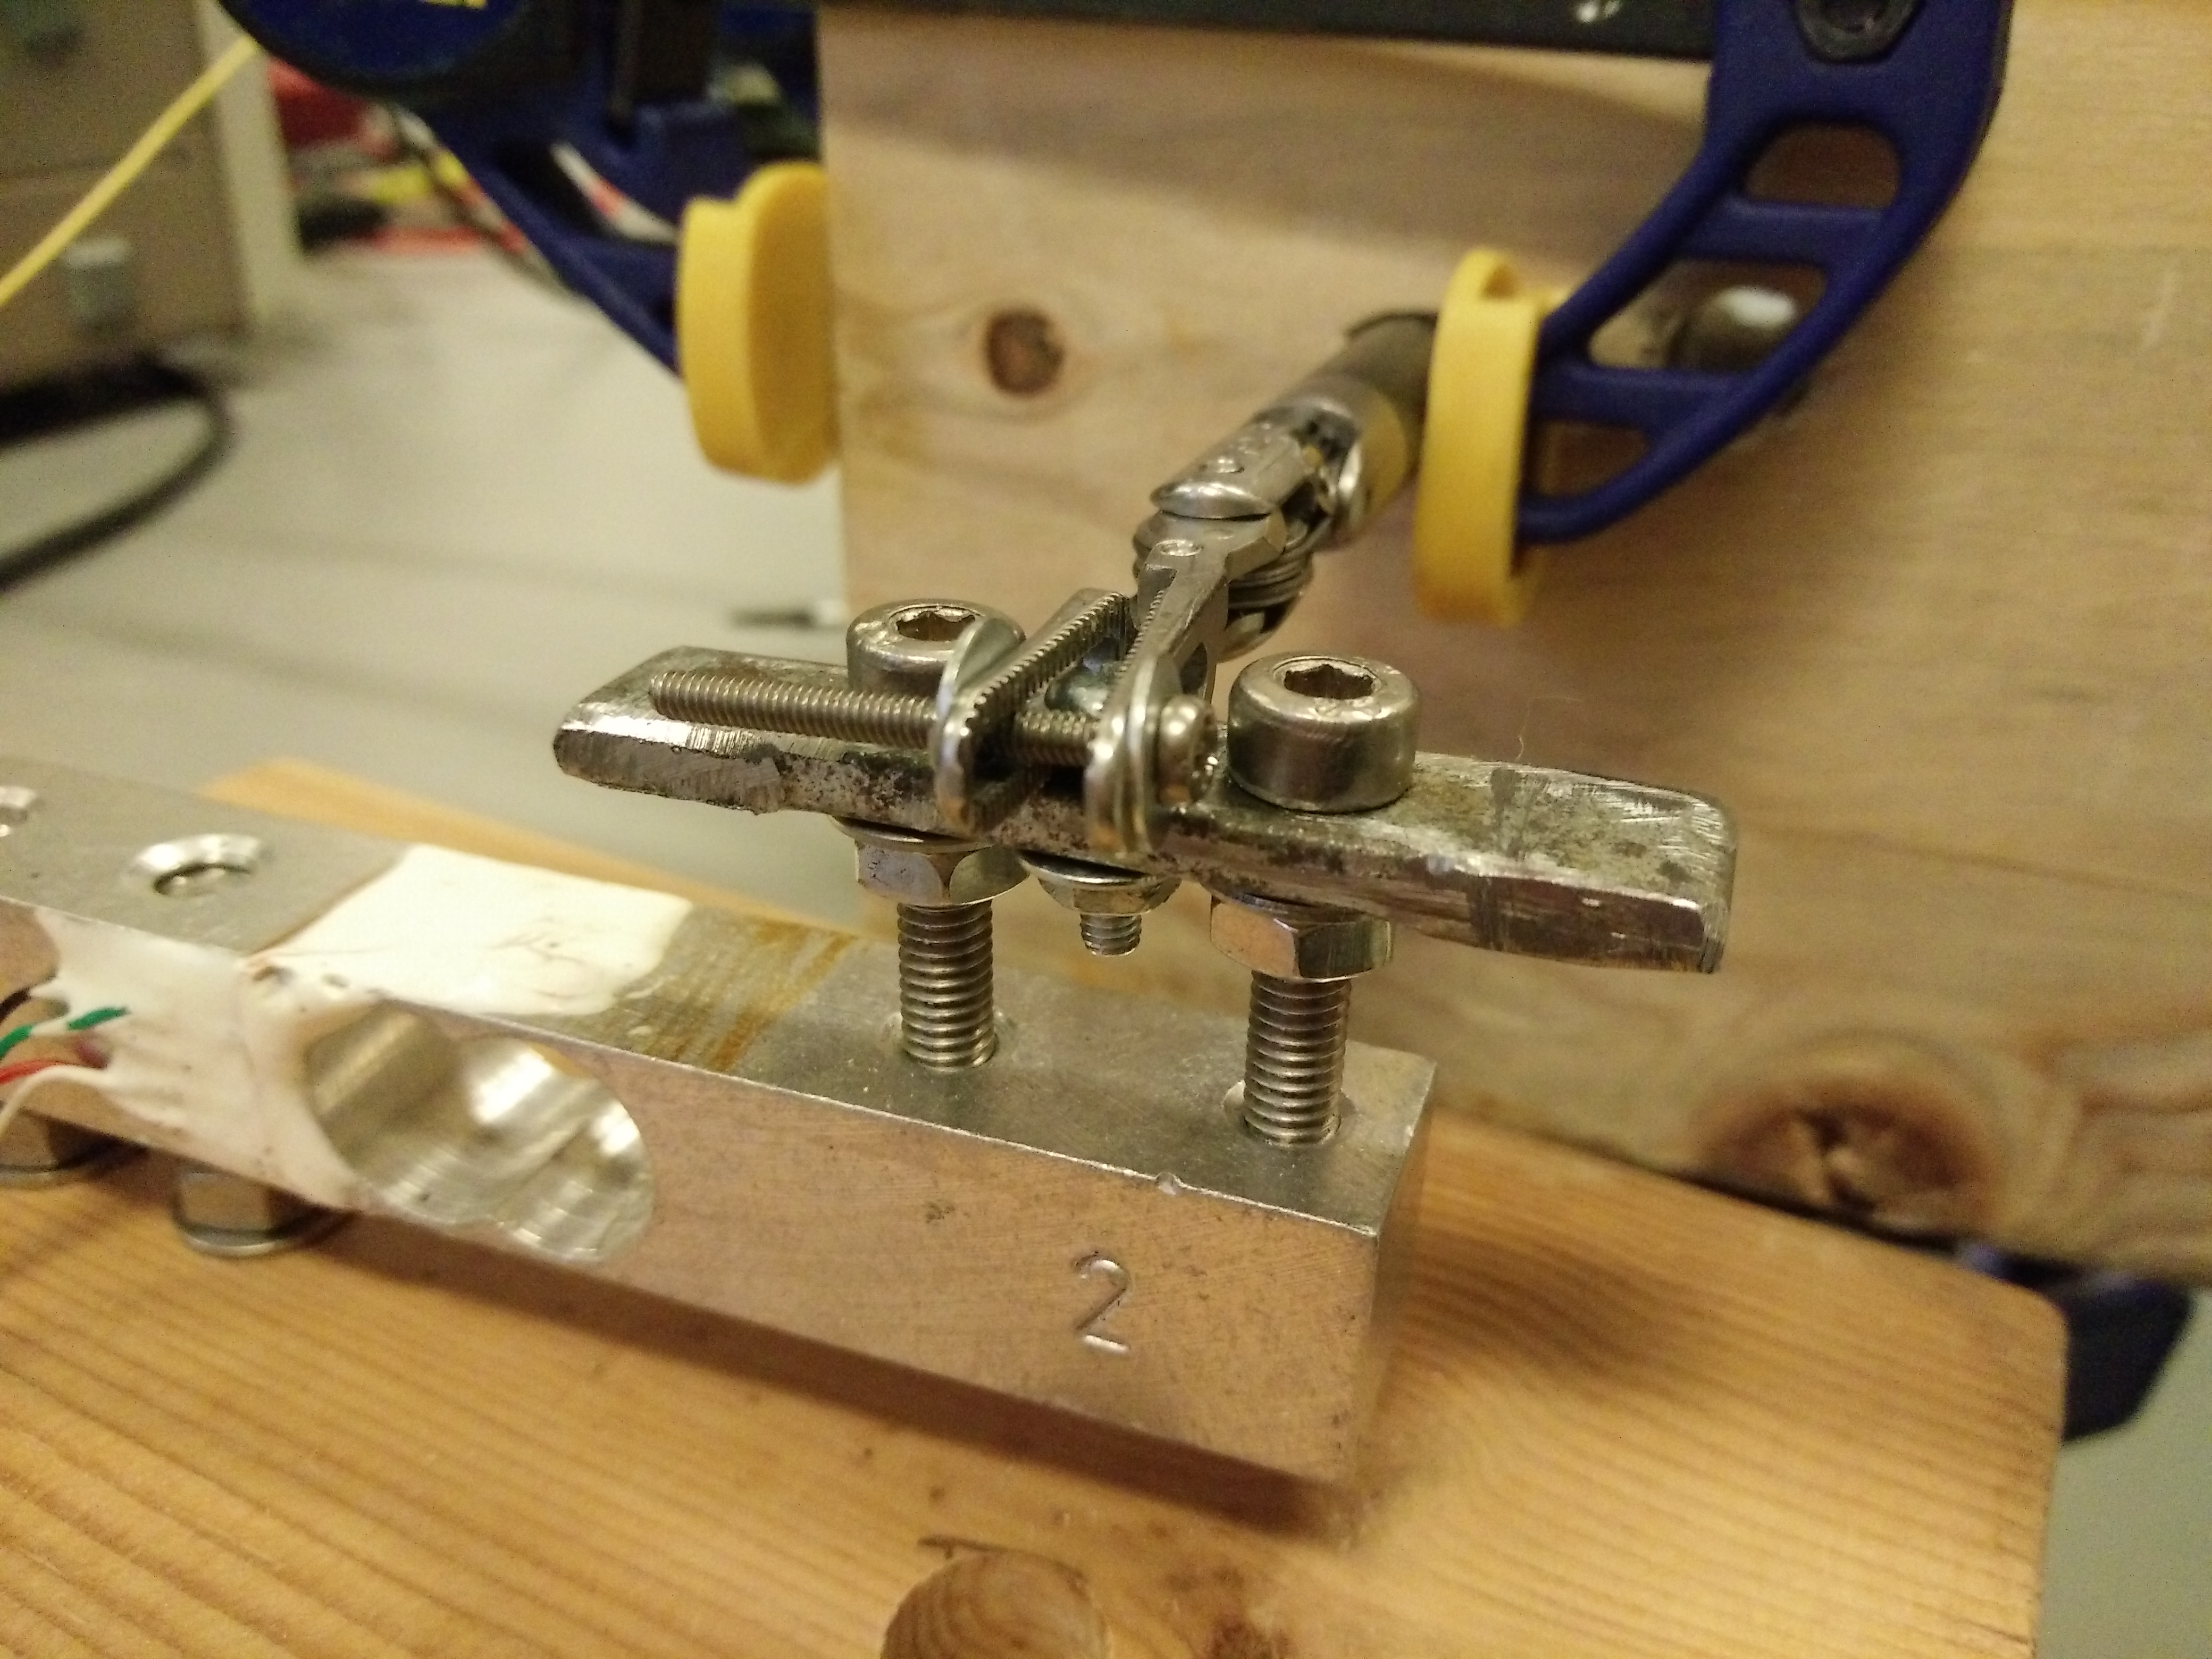
\includegraphics[width=\linewidth]{Pitch_clamp.jpg} 
        \caption{Pitch} \label{fig:mes2}
    \end{subfigure}
        \begin{subfigure}[t]{0.32\textwidth}
        \centering
        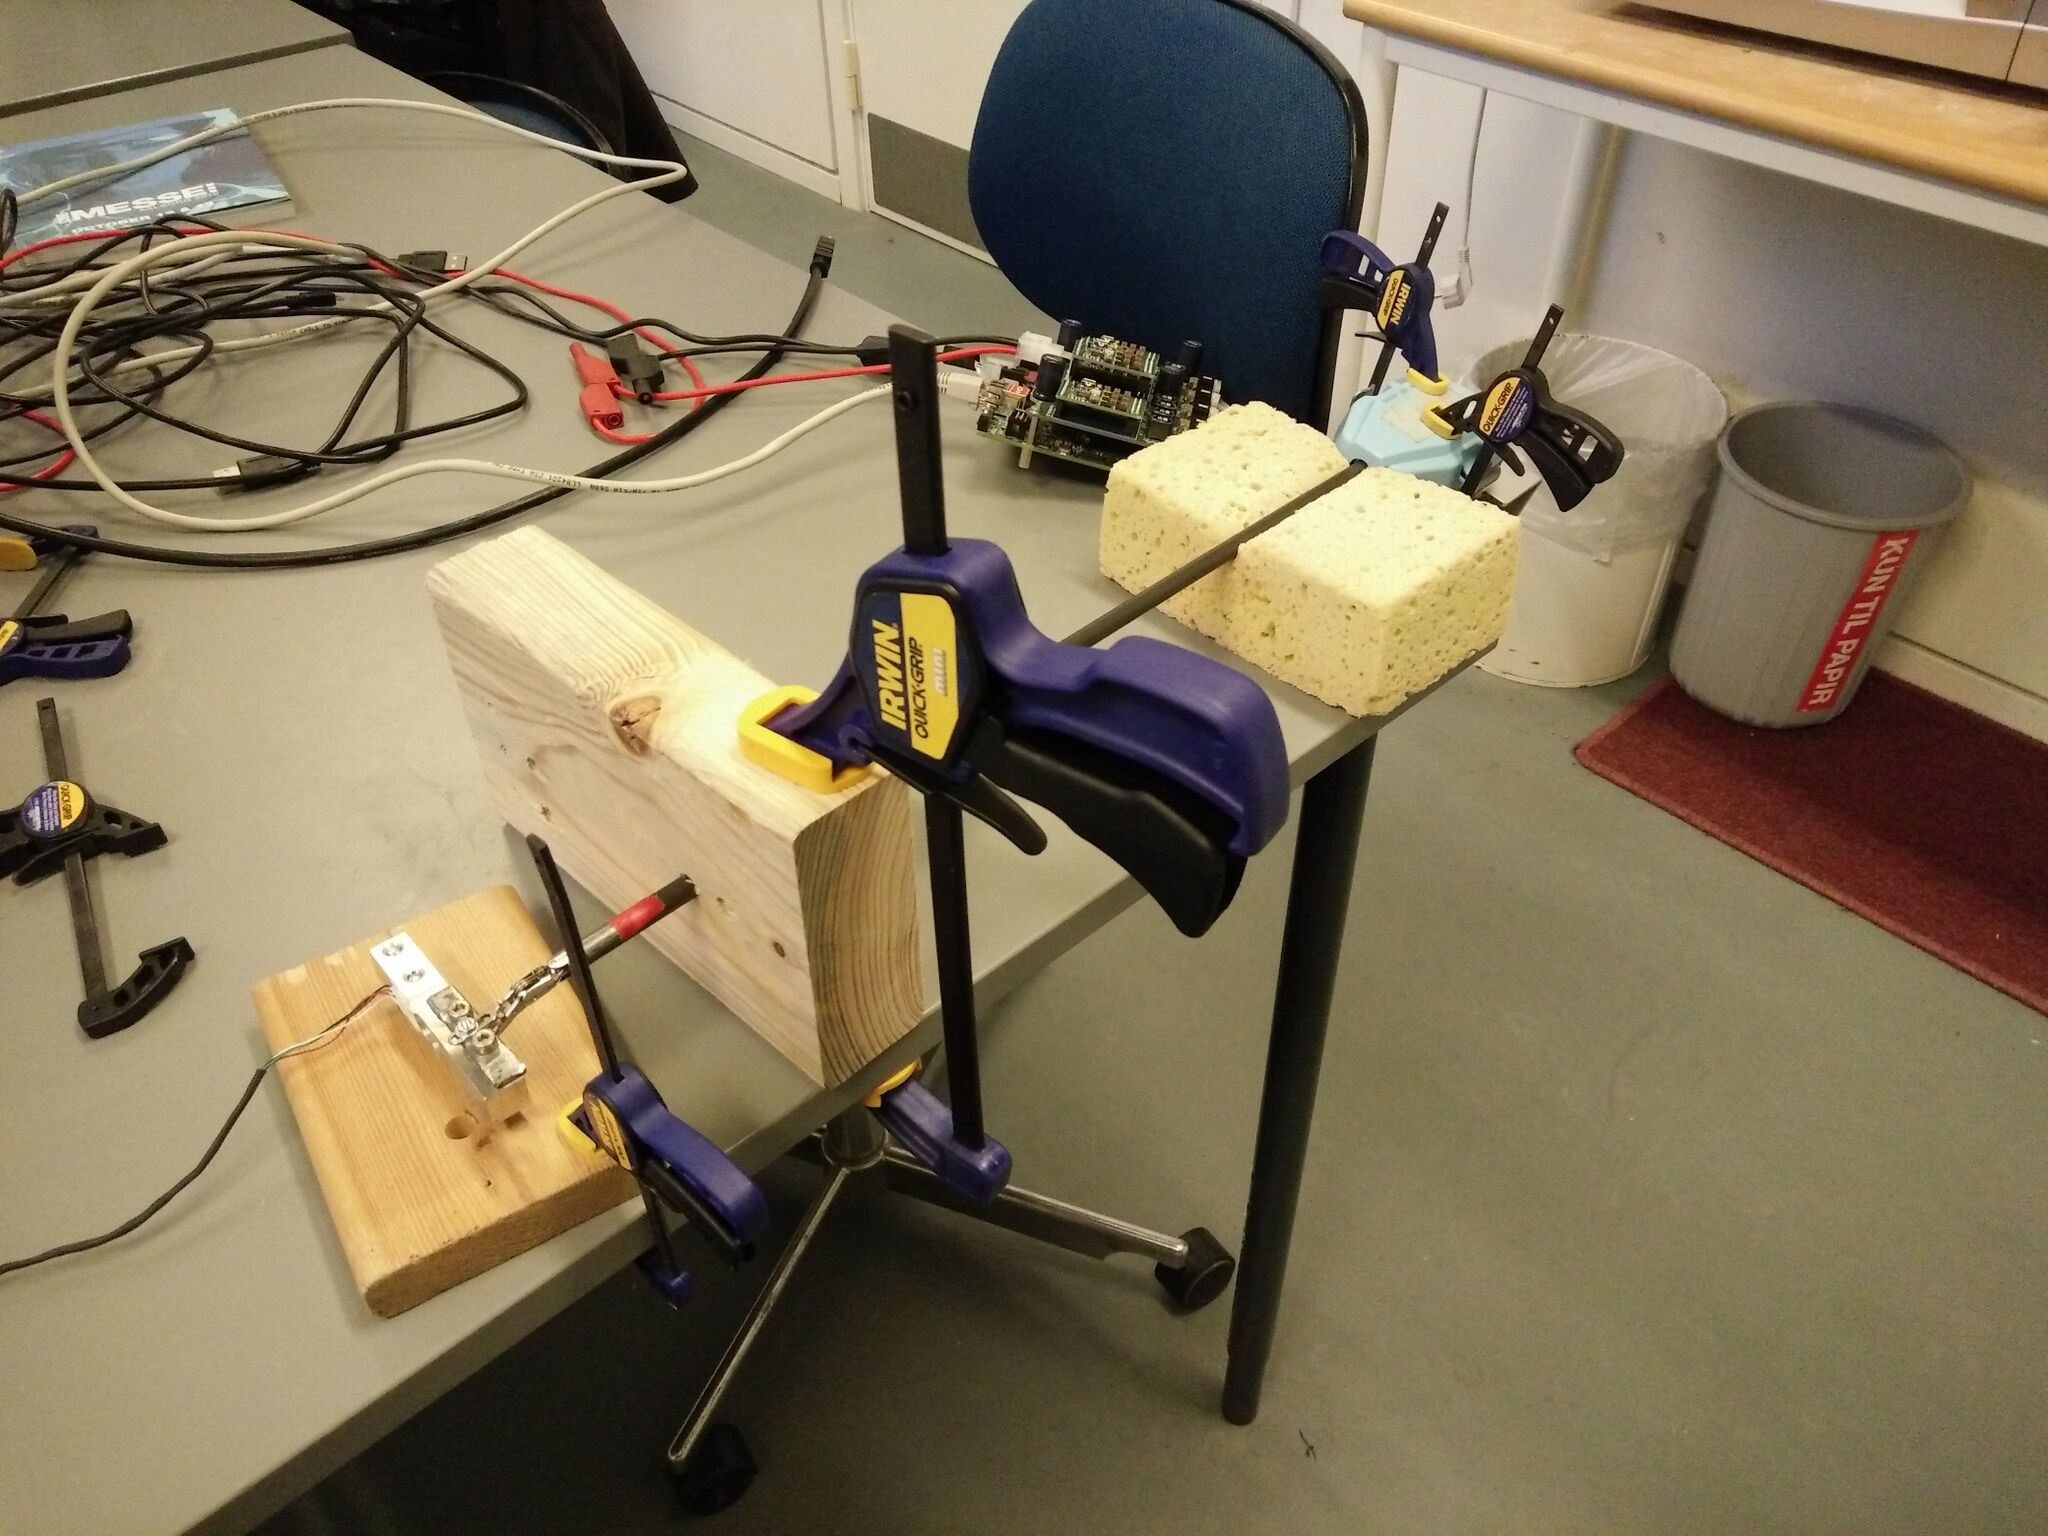
\includegraphics[width=\linewidth]{overall_force.jpg} 
        \caption{Full view} \label{fig:mes3}
    \end{subfigure}
\end{figure}
\end{frame}

\begin{frame}
\begin{itemize}
\item insert image of data
\end{itemize}
\end{frame}

% the license
\begin{frame}{Force estimation}{Model structure}

  \begin{itemize}
      \item Hammerstein-Wiener Model
	  \item Linear part is represented in state space
	  \item Nonlinearities on input and output can take different forms
	  \begin{itemize}
	  \item Deadzone, saturation ...
	  \item Neural networks
	  \end{itemize}
  \end{itemize}
%\end{column}%
%\hfill%
%\begin{column}{.65\textwidth}

\vspace{3em}
\begin{figure}[H]
\resizebox{0.9\textwidth}{!}{
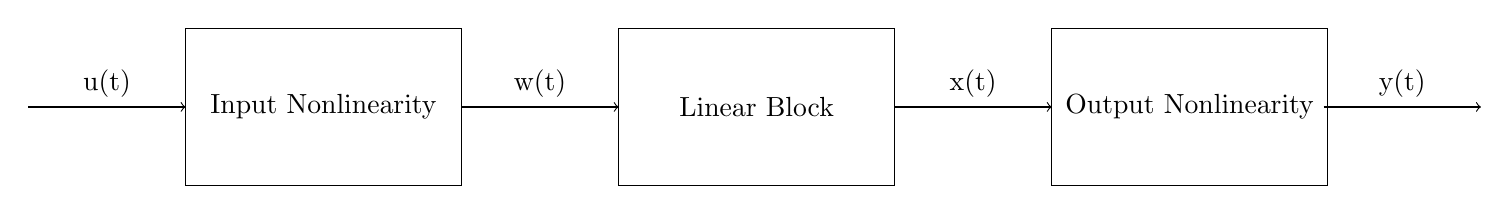
\begin{tikzpicture}
\draw  (-3.5,3) rectangle (0,1) node[pos=.5] {Linear Block};
\draw  (-9,3) rectangle (-5.5,1) node[pos=.5] {Input Nonlinearity};
\draw  (2,3) rectangle (5.5,1) node[pos=.5] {Output Nonlinearity};
\draw [->] (-5.5,2) -- (-3.5,2) node [pos=0.5,above] {w(t)};
\draw [->] (-11,2) -- (-9,2) node [pos=0.5,above] {u(t)};
\draw [->] (0,2) -- (2,2) node [pos=0.5,above] {x(t)};
\draw [->] (5.45,2) -- (7.45,2) node [pos=0.5,above] {y(t)};
\end{tikzpicture}
}
\caption{Hammerstein-Wiener model.}
\label{weiner}
\end{figure}


%\end{column}
%\end{columns}

\end{frame}



%%%%%%%%%%%%%%%%%%%%%%%%%%%%%%%%%%%%%%%%%%%%%%%%%%%%%%%%%%%%%%%%%%%%%%%%%%%%%%%%%%%

\begin{frame}{Force estimation}{Linear model}
\begin{itemize}
  \item Choice of inputs and data affects fit of model
  \item Inputs: effort, velocity 
  \item Outputs: force (, position error)
  \item Subspace identification
	\begin{itemize}
	\item Different algorithms: SSARX, CVA, MOESP
	\item Hankel singular value analysis used for picking order
	\end{itemize}
\end{itemize}
	
	\begin{figure}
	\centering
	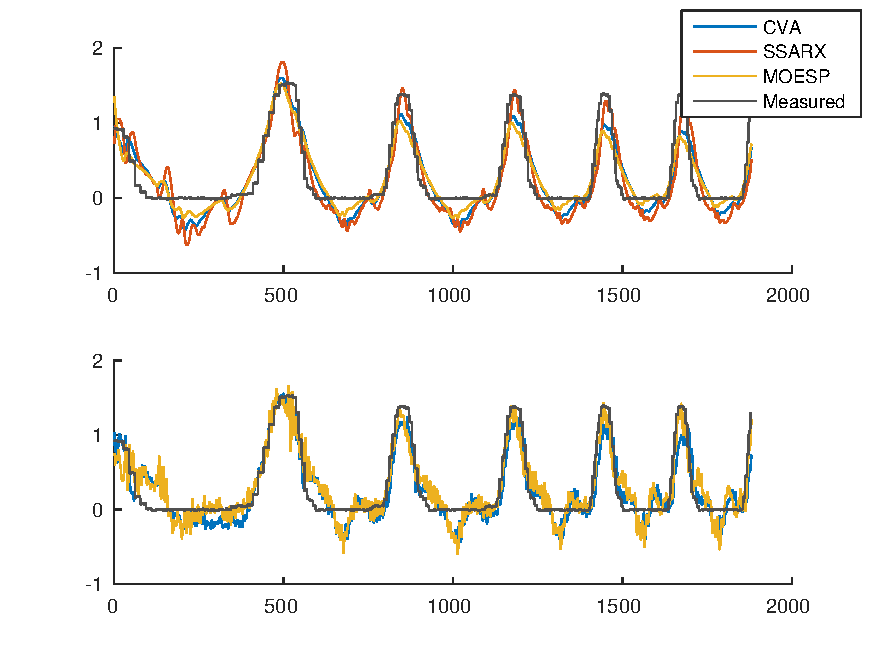
\includegraphics[width=\linewidth]{Billeder/sscomparison1-eps-converted-to.pdf}
	\end{figure}
\end{frame}

%chosen models
\begin{frame}

\end{frame}

%%%%%%%%%%

\begin{frame}{Force estimation model}{Hammerstein Wiener Models}
\begin{itemize}
  \item Nonlinearities
  \begin{itemize}
    \item Deadzone nonlinearities on input 
    \item Saturation nonlinearities on output
  \end{itemize}
\end{itemize}


 \begin{figure}[h]
 \centering
 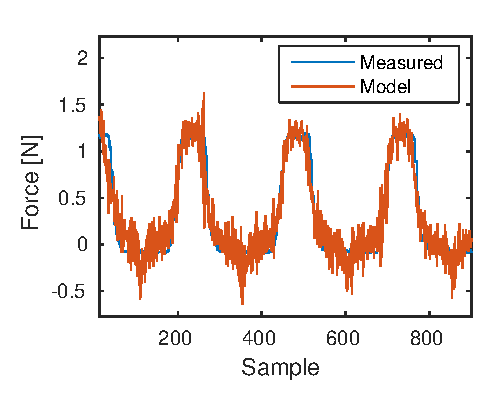
\includegraphics[width=0.49\linewidth]{modelpitch2_a}
 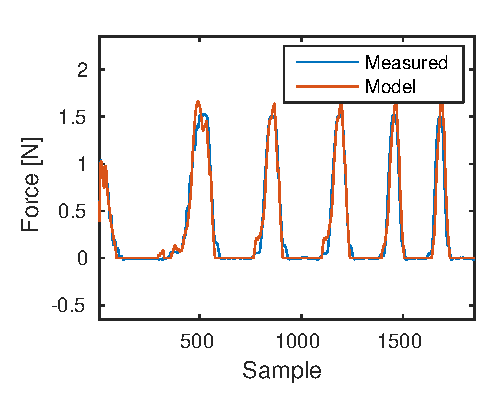
\includegraphics[width=0.49\linewidth]{modelyaw_a}
 \caption{Comparison of pitch (left) and yaw (right) model to measurements.}
 \label{fig:final_res_yaw}
 \end{figure}
\end{frame}

% in simulation part mention sliding mode control as an option to cure nonlinearities